%---------------------------------------------------------------------------%
%-                                                                         -%
%-                           LaTeX Template                                -%
%-                                                                         -%
%---------------------------------------------------------------------------%
%- Copyright (C) Huangrui Mo <huangrui.mo@gmail.com> 
%- This is free software: you can redistribute it and/or modify it
%- under the terms of the GNU General Public License as published by
%- the Free Software Foundation, either version 3 of the License, or
%- (at your option) any later version.
%---------------------------------------------------------------------------%
%->> Document class declaration
%---------------------------------------------------------------------------%
\documentclass{Style/ucasproposal}%
%- Multiple optional arguments:
%- [<oneside|twoside|print>]% oneside eprint, twoside eprint, or paper print
%- [fontset=<adobe|none|...>]% specify font set instead of automatic detection
%- [scheme=plain]% thesis writing of international students
%- [draftversion]% show draft version information
%- [standard options for ctex article class: draft|paper size|font size|...]%
%---------------------------------------------------------------------------%
%->> Document settings
%---------------------------------------------------------------------------%
\usepackage[numbers,list,xhf]{Style/artratex}% document settings
%- usage: \usepackage[option1,option2,...,optionN]{artratex}
%- Multiple optional arguments:
%- [bibtex|biber]% set bibliography processor and package
%- [<numbers|super|authoryear|alpha>]% set citation and reference style
%- <numbers>: textual: Jones [1]; parenthetical: [1]
%- <super>: textual: Jones superscript [1]; parenthetical: superscript [1]
%- <authoryear>: textual: Jones (1995); parenthetical: (Jones, 1995)
%- <alpha>: textual: not available; parenthetical: [Jon95]
%- [geometry]% reconfigure page layout via geometry package
%- [lscape]% provide landscape layout environment
%- [xhf]% disable header and footer via fancyhdr package
%- [color]% provide color support via xcolor package
%- [background]% enable page background
%- [tikz]% provide complex diagrams via tikz package
%- [table]% provide complex tables via ctable package
%- [list]% provide enhanced list environments for algorithm and coding
%- [math]% enable some extra math packages
%- [xlink]% disable link colors
\usepackage{Style/artracom}% user defined commands
%---------------------------------------------------------------------------%
%->> Document inclusion
%---------------------------------------------------------------------------%
%\includeonly{Tex/Chap_1,...,Tex/Chap_N}% selected files compilation
%---------------------------------------------------------------------------%
%->> Document content
%---------------------------------------------------------------------------%
%-
%-> Titlepage information
%-
%-> 中文封面信息
%-
\schoollogo{scale=0.112}{ucas_logo}% 校徽
\title{多架构软硬件协同二进制翻译器设计}% 题目
\author{晏悦}% 作者姓名
\authorid{202128013229037}% 学号
\advisor{王剑}% 指导老师
\advisortitle{研究员}% 指导老师职务
\degree{硕士}% 学位:硕士、博士
\degreetype{工学}% 学位类别:理学、工学、工程、医学等
\major{计算机系统结构}% 二级学科专业名称
\field{体系结构}% 研究方向
\institute{中国科学院计算技术研究所}% 院所
%\institute{中国科学院力学研究所\\流固耦合实验室}% 多行院所名称示例
%\chinesedate{2014~年~06~月}% 日期
%---------------------------------------------------------------------------%
\begin{document}
%-
%-> Frontmatter: title page, abstract, content list, symbol list, preface
%-
\pagenumbering{roman}% page numbers with roman style
% \input{Tex/Frontmatter}% title page, abstract

%---------------------------------------------------------------------------%
%-> Frontmatter
%---------------------------------------------------------------------------%
%-
%-> 生成封面
%-
\maketitle% 生成中文封面
%-
%-> 目录
%-
\tableofcontents% 生成目录
%---------------------------------------------------------------------------%
%-
%-> Mainmatter
%-
\clearpage
\pagenumbering{arabic}% restart page numbers with arabic style
% %---------------------------------------------------------------------------%
%->> Main content
%---------------------------------------------------------------------------%
\section{选题的背景及意义}

\subsection{选题背景}

关于riscv生态,以及各类指令集生态的问题。

阐述二进制翻译器的问题,以及二进制翻译器的优势。



\subsubsection{背景}


\subsection{选题意义}



\subsubsection{意义}



\section{国内外本学科领域的发展现状与趋势}



\section{课题主要研究内容、预期目标}



\section{拟采用的研究方法、技术路线、实验方案及其可行性分析}



\section{已有科研基础与所需的科研条件}



\section{研究工作计划与进度安排}



\section*{填表说明}

本表内容须真实、完整、准确。

\section*{常见使用问题}

\begin{enumerate}
    \item 模板使用说明请见 \href{https://github.com/mohuangrui/ucasthesis}{ucasthesis:中国科学院大学学位论文 LaTeX 模板}.
    \item 填表说明和模板说明不是开题报告的一部分,请删除。
    \item 开题报告样式设计导致对题目换行与不换行难以兼容,排版十分困难。推荐采用当前设置,尽量避免将精力花在这些无关紧要的细节上。
\end{enumerate}

\nocite{*}% 使文献列表显示所有参考文献(包括未引用文献)
%---------------------------------------------------------------------------%
% main content
%---------------------------------------------------------------------------%
%->> Main content
%---------------------------------------------------------------------------%

\section{学位论文进展情况、存在的问题、已取得阶段性成果}

\subsection{开题报告内容回顾}

开题报告主要介绍了本研究工作——多架构软硬协同二进制翻译器(后文统一简称为\textbf{微译器})项目。
首先介绍了研究背景——各类国产CPU有不同的指令集,各种指令集互不兼容,生态不足,
这严重阻碍了国产CPU的生态发展和市场化应用,这是生态碎片化问题;
同时常用于解决生态差异的工具(用户级二进制翻译器)难以支持多架构,同时翻译运行的效率不高,这是性能问题。

而本课题致力于解决生态碎片化问题和二进制翻译器性能问题,参考了X86处理器微码缓存的设计理念,
设计了微译器项目。

\begin{figure}[h]
  \centering
  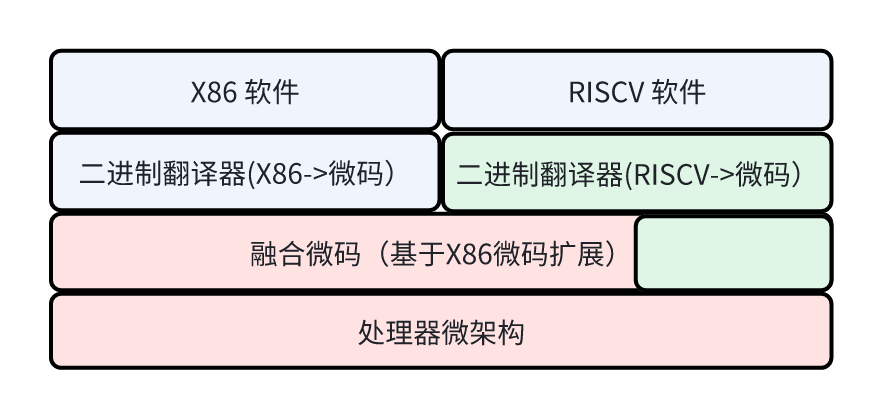
\includegraphics[width=0.8\linewidth]{./feishuImage/implement_arch.png}
  \caption{多架构软硬协同的二进制翻译架构实现图,绿色部分为本文主要工作。}
  \label{img:implement_arch}
\end{figure}

如图\ref{img:implement_arch},本文的主要工作内容为,在已有的微译器项目(已经支持X86指令集的翻译运行)上,添加RISCV多架构支持,用于验证微译器在多架构上的支持能力,
以及在跨架构上能否高效运行程序,也就是验证能否解决性能难题。



\subsection{微译器架构细节}

\begin{figure}[h]
  \centering
  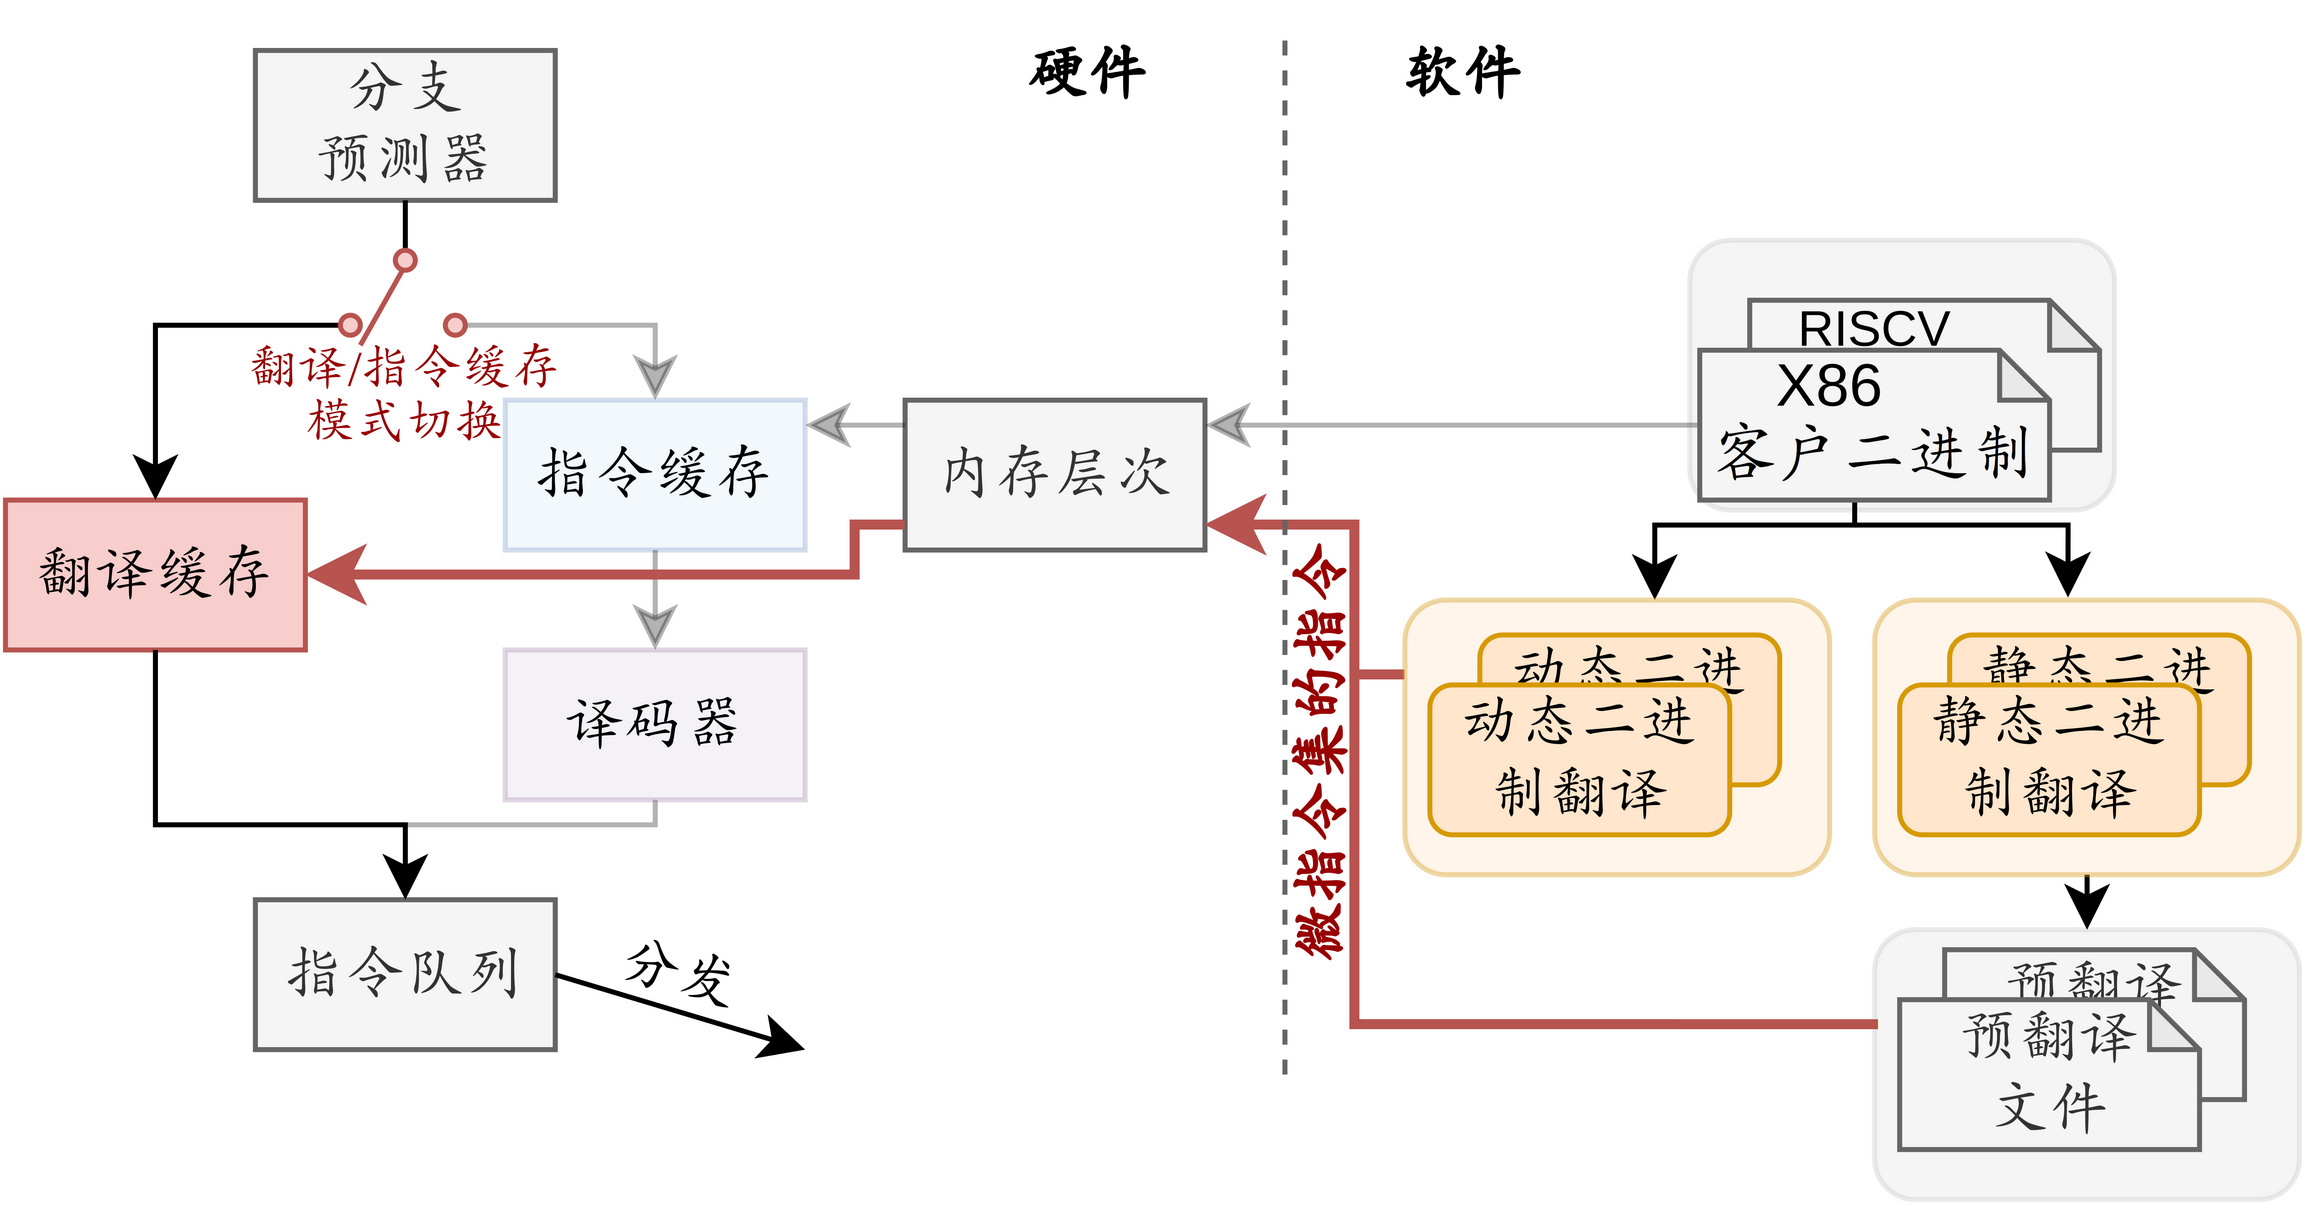
\includegraphics[width=1\linewidth]{./image/front_end_transutor.pdf}
  \caption{架构细节图。}
  \label{img:front_end_transutor}
\end{figure}

首先简要回顾一下微译器的架构细节,如图\ref{img:front_end_transutor}:

\subsubsection{硬件部分}

在硬件部分,引入了\textbf{翻译缓存}(Translation Cache),该缓存作为一级缓存负责存储预翻译的微码指令集,替代了原本的微码缓存。
翻译缓存的每行组织形式和微码缓存类似,都是前面部分存放微码指令(这里为融合微码指令,下一节详细介绍),
后面存放立即数(主要为了方便一条变长的X86指令,能更好的翻译成定长的融合微码指令),
微码指令和立即数相向生长,中间可能有空洞,这也是新产生的性能开销。

此外与传统微码架构不同,微码缓存数据是直接来源于CPU和指令缓存;
而翻译缓存通过二进制翻译透过内存层次(从内存加载到L3 Cache, 再到L2Cache, 最后到微码缓存)进行填充,
取代了传统的指令缓存和译码器的角色。
在传统X86架构下,取指部件会同时查询指令缓存和微码缓存;
而在微译器架构下,取指部件仅查询翻译缓存,硬件的译码器被软件的二进制翻译器取代。

\subsubsection{软件部分}

在软件部分,引入了静态和动态二进制翻译器。
程序首先通过静态二进制翻译器被翻译成微指令,并被写入预翻译文件,存储在硬盘中。
在客户程序执行阶段,预翻译文件被加载到内存中,程序计数器被设置为客户程序的入口。
取指部件从翻译缓存中取指,若翻译缓存或内存层次命中,则与从指令缓存取指类似,不断取指执行。
若翻译缓存和内存层次均未命中(例如存在自修改代码等),说明客户指令还未翻译,此时会调用动态二进制翻译器进行实时翻译。



\subsection{融合微码介绍}
本节详细介绍重要的一个概念——融合微码。“融合”代表它能融合了多种指令集的特征,
包括X86和RISCV,未来还可以支持ARM,MIPS等其他指令集,
或许叫统一微码也更好理解。但融合并非简单的把所有指令集简单拼接就好,这会造成指令集冗余,挤占有限的编码空间。

“微码”这个名字主要由于它在翻译缓存中的组织形式和传统的X86微码缓存组织形式类似,并且更像是不同指令集的更低级表现形式;
此外目前第一代的融合微码是在原有的Gem5 X86微码上扩充的,
所以便于理解仍然保留融合微码的名字。

但事实上,融合微码有很大特征很像一个“RISC指令集”。
由于我们的融合微码指令是需要存储在磁盘中的,并不像传统X86微码只是作为一个“暂时指令”存在于CPU运行期间,
所以融合微码指令需要像普通指令集一样进行\textbf{编码},
编译器(或者二进制翻译器)把指令\textbf{编码}为定长的融合微码指令,并存储于磁盘中。
CPU再从磁盘中加载融合微码指令,\textbf{解码}为CPU识别的信息,这一阶段也叫“译码阶段”。
因此从这个角度来说,加上指令定长、只能操作寄存器、指令间关系被简化等特征,融合微码很像一个普通的“RISC指令集”。
因此融合微码类似传统指令集概念,也是有编码空间的概念。

设计一套高效完备的融合微码“指令集”是一个长期的工程,这不是本文研究重点。
为了快速验证微译器的实际效果,同时减少“指令集设计”产生的额外性能影响,
因此目前我们的融合微码是基于在原本的Gem5 X86微码上扩充的,并谨慎的添加了部分RISCV指令,
如图\ref{img:TISA},由于X86指令默认符号扩展,而RISCV指令同时支持符号扩展和零扩展,
为了尽可能实现一条RISCV指令翻译成一条融合微码指令,所以需要添加适当的“零扩展”微码指令。

\begin{figure}[h]
  \centering
  \includegraphics[width=0.8\linewidth]{./image/TISA.pdf}
  \caption{指令翻译到融合微码过程,X86 add 和RISCV add 指令都翻译成融合微码add指令,
  而lbu(加载字节并无符合扩展)指令,需要额外添加lbu 微码指令。}
  \label{img:TISA}
\end{figure}

\subsection{RISCV指令翻译}

目前已经完成所有的RISCV指令(包括IMAFDC指令集)到融合微码的翻译。

\begin{itemize}
  \item 整数指令(I): 主要包括运算指令、逻辑指令、跳转指令、访存指令等。大部分复用X86微码,访存指令等需要额外添加新的微码。

  \item 乘除法指令(M):主要包括乘法、除法、取余等指令。大部分复用X86微码。

  \item 原子指令(A):包括原子加法、原子比较等指令。由于目前尚未实现多线程支持,
  原子加法指令被翻译为一条普通load+加法指令+一条store指令。

  \item 浮点指令(F,D):包括单精度浮点F 和双精度浮点D指令。大部分复用X86微码,出于简洁考虑,对于特殊的舍入模式暂未考虑和X86的差异。

  \item 压缩指令(C):为了压缩指令长度,把常用的4字节指令替换为2字节长度的压缩指令。尽可能把翻译得到的微码也编码为2字节。

\end{itemize}

累积统计数目如下:原本X86指令共有数千条,X86微码也有500余条。
为了添加272条RISCV指令,我们并没有简单添加272条微码指令,
而只是添加了41条整数相关指令,10条浮点相关指令,累计添加51条微码指令。

\subsection{处理ABI差异}
%介绍什么是ABI, 从而引出RISCV和X86的ABI差异。而我们的项目需要把RISCV的ABI转换成X86的ABI。
ABI全称为Aplication Binary Interface,是程序和硬件的统一接口,不同指令集的ABI也是不同的,
在二进制翻译系统中需要维护这种差异性,保证程序运行的正确性。
ABI包括内容比较多,其中主要的包括系统调用传参、初始化栈等问题,本节介绍微译器项目是如何处理ABI差异的。


\subsubsection{系统调用差异}

如表\ref{tab:syscall}所示,X86和RISCV的系统调用号和参数传递方式的差异。
X86的系统调用号存储在rax寄存器中,返回值也存储在rax寄存器中,参数传递方式为rdi, rsi, rdx, r10, r8, r9。
而RISCV的系统调用号存储在a7寄存器中,返回值存储在a0寄存器中,参数传递方式为a0, a1, a2, a3, a4, a5。
因此我们需要在RISCV的二进制翻译器中,将RISCV的系统调用号和参数传递方式转换成X86的系统调用号和参数传递方式。

参数传递的差异可以通过把X86的参数寄存器和RISCV的参数寄存器映射到相同的微码寄存器即可,如表\ref{tab:reg_map}所示,
所有的黄色寄存器就是6个参数传递寄存器。系统调用号差异同理也可解决。


\begin{table}[]
  \centering
  \caption{
    X86和RISCV的系统调用号和参数传递方式的差异。
  }
  \label{tab:syscall}
  \begin{tabular}{llllllllll}
  \rowcolor[HTML]{FFCC67} 
  \cellcolor[HTML]{FBE5D6}指令集 & \cellcolor[HTML]{FBE5D6}系统调用号 & \cellcolor[HTML]{FBE5D6}返回值 & 参数1 & 参数2 & 参数3 & 参数4 & 参数5 & 参数6 & 其他参数 \\
  X86                         & rax                           & rax                         & rdi & rsi & rdx & r10 & r8  & r9  & 栈传递  \\
  RISCV                       & a7                            & a0                          & a0  & a1  & a2  & a3  & a4  & a5  & 栈传递 
  \end{tabular}
  \end{table}


\subsubsection{寄存器映射表}

寄存器映射一直是二进制翻译中一个重要的研究课题。
如表\ref{tab:reg_map}所示,展示了X86和RISCV映射到微码的的寄存器映射表。
对于X86寄存器映射到微码寄存器较为容易,因为X86只有16个通用整数寄存器,而微码我们定义了32个通用寄存器,
所以只需要把X86寄存器固定映射到前16个通用寄存器即可,还可以把一些常用的寄存器
(例如AH,BH等子寄存器和段寄存器)映射到后面的寄存器中,还可用一些寄存器作为临时寄存器供二进制翻译器使用。

但是对于RISCV映射到微码方案,由于RISCV本身就有32个通用寄存器,固定映射到32个微码寄存器后,
就没有额外的临时寄存器供二进制翻译器使用了。对于微译器项目,得益于软硬件协同设计的基本原则,
我们额外添加了两个微码寄存器作为临时寄存器,
这两个寄存器只对二进制翻译器可见,不对RISCV应用程序可见,类似于X86“段寄存器”,属于特殊寄存器。



\begin{table}[]
  \centering
  \caption{
    X86和RISCV的寄存器映射表。
  }
  \label{tab:reg_map}
  \begin{tabular}{|
    >{\columncolor[HTML]{FFCCC9}}l |l|l|
    >{\columncolor[HTML]{FFCCC9}}l |
    >{\columncolor[HTML]{FFFFFF}}l |
    >{\columncolor[HTML]{FFFFFF}}l |
    >{\columncolor[HTML]{FFCCC9}}l |
    >{\columncolor[HTML]{FFFFFF}}l |
    >{\columncolor[HTML]{FFFFFF}}l |
    >{\columncolor[HTML]{FFCCC9}}l |
    >{\columncolor[HTML]{FFFFFF}}l |
    >{\columncolor[HTML]{FFFFFF}}l |}
    \hline
    \cellcolor[HTML]{FBE5D6}微码 & \cellcolor[HTML]{FBE5D6}X86 & \cellcolor[HTML]{FBE5D6}RISCV & \cellcolor[HTML]{FBE5D6}微码 & \cellcolor[HTML]{FBE5D6}X86 & \cellcolor[HTML]{FBE5D6}RISCV & \cellcolor[HTML]{FBE5D6}微码 & \cellcolor[HTML]{FBE5D6}X86 & \cellcolor[HTML]{FBE5D6}RISCV & \cellcolor[HTML]{FBE5D6}微码 & \cellcolor[HTML]{FBE5D6}X86 & \cellcolor[HTML]{FBE5D6}RISCV \\ \hline
    0                          & \cellcolor[HTML]{FFFC9E}RAX & \cellcolor[HTML]{FFFC9E}A7    & 8                          & \cellcolor[HTML]{FFFC9E}R8  & \cellcolor[HTML]{FFFC9E}A4    & 16                         & T0                          & Zero                          & 24                         & CH                          & S8                            \\ \hline
    1                          & \cellcolor[HTML]{FFFFFF}RCX & \cellcolor[HTML]{FFFFFF}TP    & 9                          & \cellcolor[HTML]{FFFC9E}R9  & \cellcolor[HTML]{FFFC9E}A5    & 17                         & T1                          & RA                            & 25                         & DH                          & S9                            \\ \hline
    2                          & \cellcolor[HTML]{FFFC9E}RDX & \cellcolor[HTML]{FFFC9E}A2    & 10                         & \cellcolor[HTML]{FFFC9E}R10 & \cellcolor[HTML]{FFFC9E}A3    & 18                         & T2                          & S2                            & 26                         & ES                          & S10                           \\ \hline
    3                          & \cellcolor[HTML]{FFFFFF}RBX & \cellcolor[HTML]{FFFFFF}GP    & 11                         & R11                         & A6                            & 19                         & T3                          & S3                            & 27                         & CS                          & S11                           \\ \hline
    4                          & \cellcolor[HTML]{FFFFFF}RSP & \cellcolor[HTML]{FFFFFF}SP    & 12                         & R12                         & T1                            & 20                         & T4                          & S4                            & 28                         & SS                          & T3                            \\ \hline
    5                          & \cellcolor[HTML]{FFFFFF}RBP & \cellcolor[HTML]{FFFFFF}T0    & 13                         & R13                         & T2                            & 21                         & T5                          & S5                            & 29                         & DS                          & T4                            \\ \hline
    6                          & \cellcolor[HTML]{FFFC9E}RSI & \cellcolor[HTML]{FFFC9E}A1    & 14                         & R14                         & S0                            & 22                         & AH                          & S6                            & 30                         & FS                          & T5                            \\ \hline
    7                          & \cellcolor[HTML]{FFFC9E}RDI & \cellcolor[HTML]{FFFC9E}A0    & 15                         & R15                         & S1                            & 23                         & BH                          & S7                            & 31                         & GS                          & T6                            \\ \hline
    \end{tabular}
    \end{table}

% \subsubsection{栈的初始化}
% 由于我们目前关注于用户态二进制翻译器,不太涉及系统态指令的翻译和处理操作系统等概念,
% 但是当加载运行不同指令集的程序时,在libc库眼中,操作系统已经准备好了这个程序的初始化栈等信息,例如argc,argv参数、
% 环境变量指针等,对于X86和RISCV程序,这个初始化栈是不同的,需要不同的处理


\section{实验数据分析}


\section{下一步工作计划和内容、预期答辩时间}

以下为本课题的下一步工作计划与进度安排:

\begin{itemize}
  \item 2024年2月-2024年2月:修复所有指令翻译的问题,目标成功运行SPEC CPU 2000所有子项目(整数和浮点程序的test子项)。
  \item 2024年3月-2024年3月:优化RISCV 到微码的指令编码继续压缩,减少每条指令平均长度。同时添加微码缓存预取机制,降低微码缓存缺失率。
  \item 2024年4月-2024年4月:整理数据,撰写硕士毕业论文。
\end{itemize}

预期在2024年夏季准时参加硕士答辩。


\section{已取得研究成果列表(已发表、待发表学术论文、专利等)}

目前作为第二作者,已经发表论文一篇(CCF A类TACO期刊),待发表论文一篇,没有发表专利。

已发表的论文的主要研究主流二进制翻译器的动态运行指令膨胀率,指令膨胀率和翻译后性能下降成正比,
所以分析指令膨胀率的主要来源就能定位到翻译器的性能开销,进而优化二进制翻译器的设计。
我们设计了一个高效且准确的指令膨胀分析模拟器,对于
苹果的Rosetta2\cite{RosettaTranslationEnvironment, RunningIntelBinaries}、
华为的ExaGear\cite{KunPengExaGear}、
和龙芯的LATX\cite{LoongArchEnv2022, LoongArch2023}
模拟准确度都在5\%以内,能很好的定位到性能来源。
这也是本篇硕士论文的理论基础,正是分析到了这些性能开销,才引导我们设计了这个高效率、多架构、软硬协同二进制翻译器项目。

待发表的论文基本就是本篇硕士论文的研究内容,同时更详细的介绍了微译器项目的整体框架和X86指令的支持情况,
本篇硕士论文可以作为这篇待发表论文的重要组成部分。


% \nocite{*}% 使文献列表显示所有参考文献(包括未引用文献)
%---------------------------------------------------------------------------%



%-
%-> Backmatter: bibliography, glossary, index
%-
\artxifstreq{\artxbib}{bibtex}{% enable bibtex
    \bibliography{./kaiti.bib}% bibliography
}{%
    \printbibliography% bibliography
}
\end{document}
%---------------------------------------------------------------------------%

